\section{The Design} 
\emph{etherSound} is an attempt to open a musical work to the un-initiated listener, including him or her in the creation of the music, and provide for a notion of `equality of participation': all contributions are equally valuable. Accessibility without prior knowledge of music or musical training is an end in itself in this project. It should be noted that this obviously presupposes that the participant knows how to send an SMS and that the system makes it difficult for those who are not familiar with this technology.\footnote{At the time this project was initiated, however, there was great commercial interest in increasing the use of SMS and in Sweden there has been a concerted effort on the part of the GSM service providers to teach their customers how to use it.} It should also be made clear that using SMS text messages for interaction, as implemented here, does not allow for direct dynamic control. Every message generates one `message-composition' and all control data are derived from the content of the message.

\begin{figure}[hbp]
\begin{center}
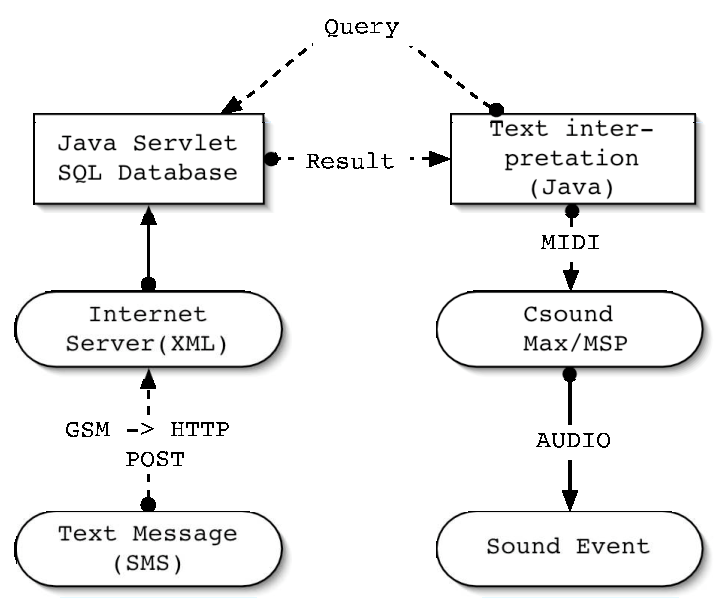
\includegraphics[width=0.45\textwidth]{img/ethsnd/Figure1}
\caption{Communication in the first version.} \label{model1}
\end{center}
\end{figure}

\subsection{Communication---first model}
\label{sec:comm-first}
In the first version, realised in August 2003,\footnote{See the audio   and video recording \emph{etherSound}/\emph{etherSound 2003}.} the communication between the participant and the system was accomplished according to \hyperref[model1]{Figure \ref*{model1}}. An SMS sent to a specified number was transformed to an XML file (eXtensible Markup Language, see \url{http://en.wikipedia.org/wiki/XML}) and transferred to a URL by an HTTP POST request. This part was handled through an external service. At the called URL, a JSP (Java Server Pages)  directed the POST data to a Java Bean\footcite{j2ee} that handled the parsing of the data and the connection to a MySQL database in which it created a new entry with the relevant fields. 

It was owing to security reasons at the museum where this version was realised that the HTTP request could not be handled locally. Instead, the local computer queried the server database for new entries on regular intervals.  After some testing, sending a SQL query once every second seemed like a reasonable time interval. Shorter time intervals did not accomplish a perceivably quicker response time and, since the synthesis program was running on the same machine, I did not want to use more processing and network activity than was necessary for this task. After the text message had been processed, control signals were sent by \useGlosentry{glos:MIDI}{MIDI} to the synthesis engine. 

As is obvious from the recordings of the two versions, the sounds produced by the computer in this first version are very different from those in the second recording.

\begin{figure}[hbp]
  \begin{center}
    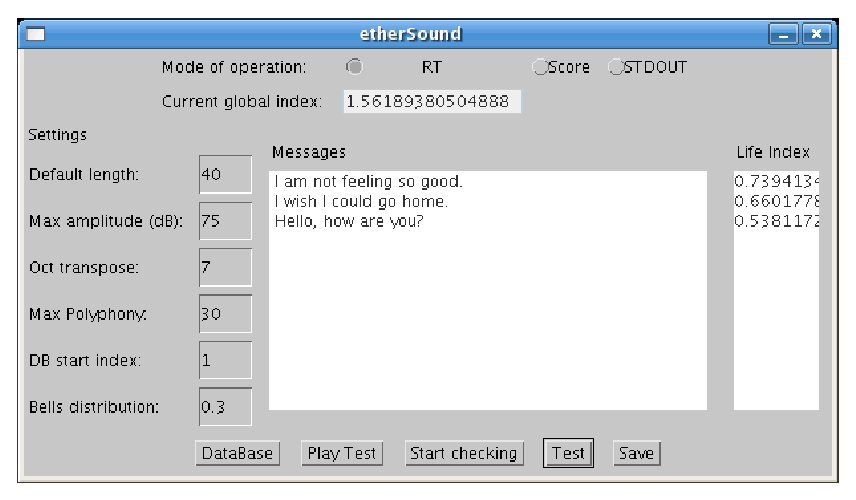
\includegraphics[width=0.9\textwidth]{img/ethsnd/MainGUI}
  \caption{Main GUI window for the \emph{etherSound} program.}
  \label{fig:main_gui}
\end{center}
\end{figure}

\subsection{Communication---current model}
Although the first version worked well and was fairly stable, it was a solution that required an external SMS processing service, and a local, reliable network connection. In order to make the piece more `portable' and independent, the message-receiving part was rebuilt. Using the gnokii API\footcite{gnokii} it is relatively easy and reliable to connect a GSM phone to a computer and gain access to the storage and status of the phone which enable reception of the SMS messages locally. To retain the possibility of reviewing the activities of transmission, the messages are, just as in the first model, written to a database. In other words, the client-server model is retained but on one and the same machine. Furthermore, the MIDI connection between the control application and the synthesis engine was replaced with \index{Open Sound Control}\index{OSC}Open Sound Control (\useGlosentry{glos:OSC}{OSC})\footcite{osc, osc_web} for speed, reliability and flexibility, using the library JavaOSC.\footnote{See \url{http://www.mat.ucsb.edu/~c.ramakr/illposed/javaosc.html}.}

\begin{figure}[hbp]
  \centering
  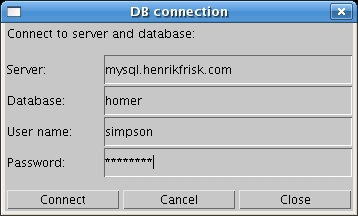
\includegraphics[width=0.5\textwidth]{img/ethsnd/DB_connection_window}
  \caption{Panel for connecting to the database.}
  \label{fig:DBpane}
\end{figure}

\subsection{The text analysis}
The program handling the text processing and the mapping of text to control signals for the sound synthesis is written in Java \footcite{j2se} and features a simple but useful Graphical User Interface  \index{GUI (Graphical User Interface)}GUI) for control and feedback about the status of the system (see Figure \ref{fig:main_gui} and Figure \ref{fig:DBpane}).  

% It is in the mapping % between the text and the synthesis and sequencing of the sound events % that the musical potential of the system is constructed.  From the information extracted from the message control signals are generated which then influence (ordered from general to specific): 
\begin{itemize}
\item{The length of the whole event}
\item{The rhythm and articulation of the individual sound events}
\item{The pitch and character of individual sound events}
\end{itemize}
There are two parameters controlling the timing of events; a local `life' index shaping the rhythms and the length of the current message and a global index that influences the current and subsequent `message-compositions'. The global index is a function of the current and previous messages local indexes. The local index is a result of a simple semantic analysis of the message. It indicates the message's relative structural complexity and allows the algorithm to discriminate between messages with a set of random letters and messages with real words and real sentences. The participant should be rewarded for the effort of writing a message with substance, where `substance' is defined here as a message with a credible average word length and a reasonable distribution of vowels within these words. In the analysis substitutions are made to allow for (i.e. not punish) idiomatic SMS writing such as `R u here?' or `C u 2 nite'. These examples are expanded into their `correct' equivalent. Standard abbreviations are also expanded. 

The local index is calculated by looking at the average length of words and the average number of syllables per word and comparing these with constants: 

\begin{equation}\label{index}
i_1=\frac{1}{(w(\frac{c}{w_c})-w_l)^{1/2}+1} \qquad i_2=\frac{1}{(w(\frac{s}{w_c})-s_l)^{1/2}+1}
\end{equation}

where $c$ and $s$ are the total number of characters and syllables, $w_c$ is the number of words in the current message and $w_l$ and $s_l$ are constants defining the `optimal' mean number of words/syllables. $w$ is a weight defined by 
\begin{equation}
w=\frac{1}{w_c-s_c+0.5}
\end{equation}

where $s_c$ is the total number of words that contain vowels. Through $w$, the index is decreased if the message contains words without vowels. The mean value of $i_1$ and $i_2$ is then multiplied by the arcus tangens of the number of words in relation to a third constant parameter, $o_w$, delimiting the optimal number of words per message\footnote{Since an SMS is limited to 160 characters these   constants are set according to what kind of message content should   be rewarded.} according to \eqref{life}.

\begin{equation} \label{life}
lifeIndex = \frac{i_1+i_2}{2}{\arctan (\frac{w_c}{o_w})}
\end{equation}

If we set $w_l$ to 4.5, $s_l$ to 2.0 and $o_w$ to 10 the result in four different messages can be seen in Table \ref{result}; the method distinguishes fairly well between nonsense and real words at a low computational cost. Similar or better results could conceivably be achieved in a number of different ways but this method appears to work well for the purpose.

  \begin{table}[!tbp]
    \begin{center}
      \begin{tabular}{l|r}
        \hline
        \textbf{Message} & \textbf{Life index} \\
        \hline
        \small{hello} & 0.18882 \\
        \hline
        \small{\textit{Hello, my name is Henrik}} & \textit{0.81032} \\
        \hline
        \small{hjdks la s duyfke jhsldf hasdfiw uehr jkdsl} & 0.14448 \\
        \hline
        \small{\textit{From fairest creatures we desire increase,}} & \textit{1.44618} \\
        \small{\textit{\ \ \ \ That thereby beautys rose might never}} & \\
        \hline
      \end{tabular}
      \caption{Life index for four different messages.} \label{result}
    \end{center}
  \end{table}

  The total length of the music derived from the message is calculated   by multiplying a constant preset time with the local index. Any new   message received adds its local index to the instantaneous global index which decreases exponentially at a set rate.\footnote{The rate is context-dependent. In a performance with improvisation it would be shorter than in an installation.} If a message causes the global index to reach maximum, it stops the playback of the current   message and begins playing back a pre-composed pattern, sonically   different from the output of a typical message, for about 30 seconds   before resuming ordinary mode and starts playing back the message   that caused the break. This feature is added to reward collaborative   efforts. The global index mainly controls the density and the   overall volume of the output, but also the distribution of random   and stochastic processes in the synthesis. 

\subsection{The synthesis}

The synthesis engine is written as a \useGlosentry{glos:csound}{Csound} orchestra.\footcite{csound} \footnote{For more information on Csound see also \url{http://www.csounds.com/}} In the first versions of \emph{etherSound} Csound was running inside a \index{Max/MSP}Max/MSP (\url{http://www.cycling74.com/products/maxmsp.html}) patch through the use of the \texttt{csound$\sim$} object (see \url{http://www.csounds.com/matt/}). The Csound score for the message to be played back was sent to \index{Max/MSP}Max/MSP using \useGlosentry{glos:OSC}{OSC}. \useGlosentry{glos:Max}{Max/MSP} was responsible for timing the note events and preparing valid information for the \texttt{csound$\sim$} object and the orchestra file associated with it. Owing to processing power limitations only one message could be played back simultaneously; if a message was received before the previously received message had finished playing back, the new message would interrupt the current message (this can be clearly heard in the recording of the performance from 2003). In the latest version of the \emph{etherSound} \index{software}software, instead of sending the Csound score events being sent over OSC, they were sequenced and written to the standard output and sent to Csound through a UNIX pipe. Also, rather than the number of voices being limited by new messages crudely cutting off currently playing messages, the number of simultaneous voices available is now set in the \emph{etherSound} \index{GUI (Graphical User Interface)}GUI (see Figure \ref{fig:main_gui}) and may be changed dynamically. The following discussion relates to the current version of \emph{etherSound}. 

\begin{figure}[!hbp]
  \centering
  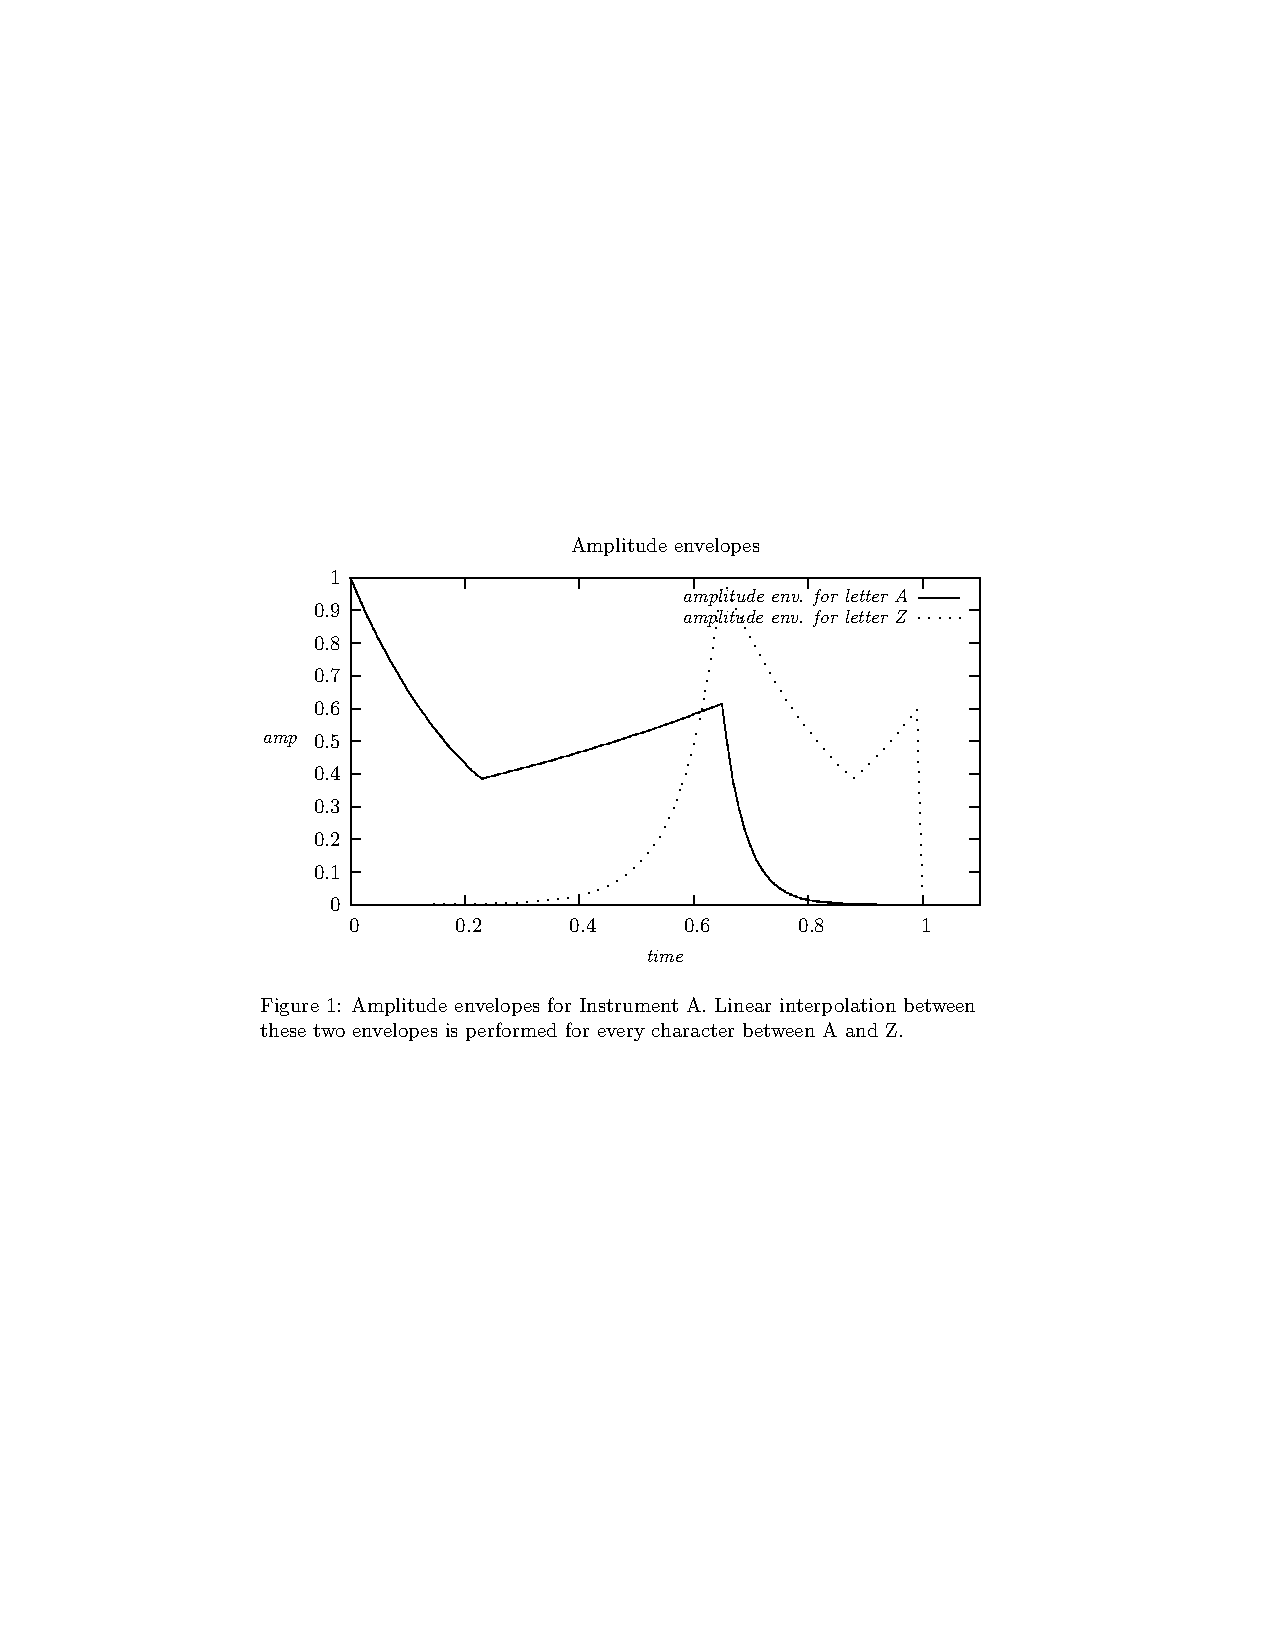
\includegraphics[trim=40mm 120mm 0mm 80mm, clip, height=50mm]{img/ethsnd/envelope}
  \caption[Amplitude envelopes for \emph{etherSound}: Instrument A.]{Amplitude envelopes for Instrument A. Linear interpolation
    between these two envelopes is performed for every character
    between A and Z.}
  \label{fig:envelope}
\end{figure}

All sounds heard in \emph{etherSound} are generated with FOF (Fonction d'Onde Formantique) synthesis, as this technique is implemented in Csound,\footcite{fof,fof2}, using both samples and simple sine waves as sound sources. There are two distinct timbres played by two different instruments in each message-composition: (A) granulated samples of a male reading a text in English\footnote{An excerpt from the recording of one of John Cage's lectures at Harvard College 1989.} and (B) a bell-like sound whose formants are matched to and interpolated between the series of vowels in the text.  

\subsubsection{Instrument A} Every word of the message is considered as one phrase or \emph{bar} of music in the resulting message composition. The number of beats per bar is approximately equal to the number of syllables in the word, where a syllable is defined as a vowel or group of consecutive vowels or a punctuation mark. The rhythmic subdivision of each bar is equal to the number of characters, including punctuation and white space, in each syllable. Thus, a monosyllabic word such as `my' followed by a white space results in a phrase consisting of one bar of one beat and two notes and one pause, i.e. three (eight-note) triplets of which the last is silent (see Table \ref{time}). If a word ends with a full stop, a comma, an exclamation mark or a question mark, more emphasis is put on the end of the bar containing the punctuation mark and the last note of the resulting phrase will be elongated. A note close to a vowel is more likely to be accented than a note further away from a vowel. 

The amplitude envelope curve of each note is related to the letter to which the note corresponds. Envelopes are mapped linearly to characters; the letter `A' has a short attack and a long decay and the letter `Z' has a long attack and a short decay (see Figure \ref{fig:envelope}). The amount of overlapping between notes, i.e. the lengths of the notes, is influenced by the current life index \emph{and} the global index where higher values will result in longer notes and thus in smoother transitions between timbres. The notes of Instrument A do not have a perceivable pitch. Twenty-eight short sample buffers (typically 32.768 samples or approximately 0.7 seconds), one for each letter, are dynamically mapped one to one to the characters in each message. The FOF synthesis is used to granulate these samples, creating an erratic, non-tonal texture but still, in most cases, reminiscent of speech. 
\begin{figure}[!htb]
  \begin{center}
    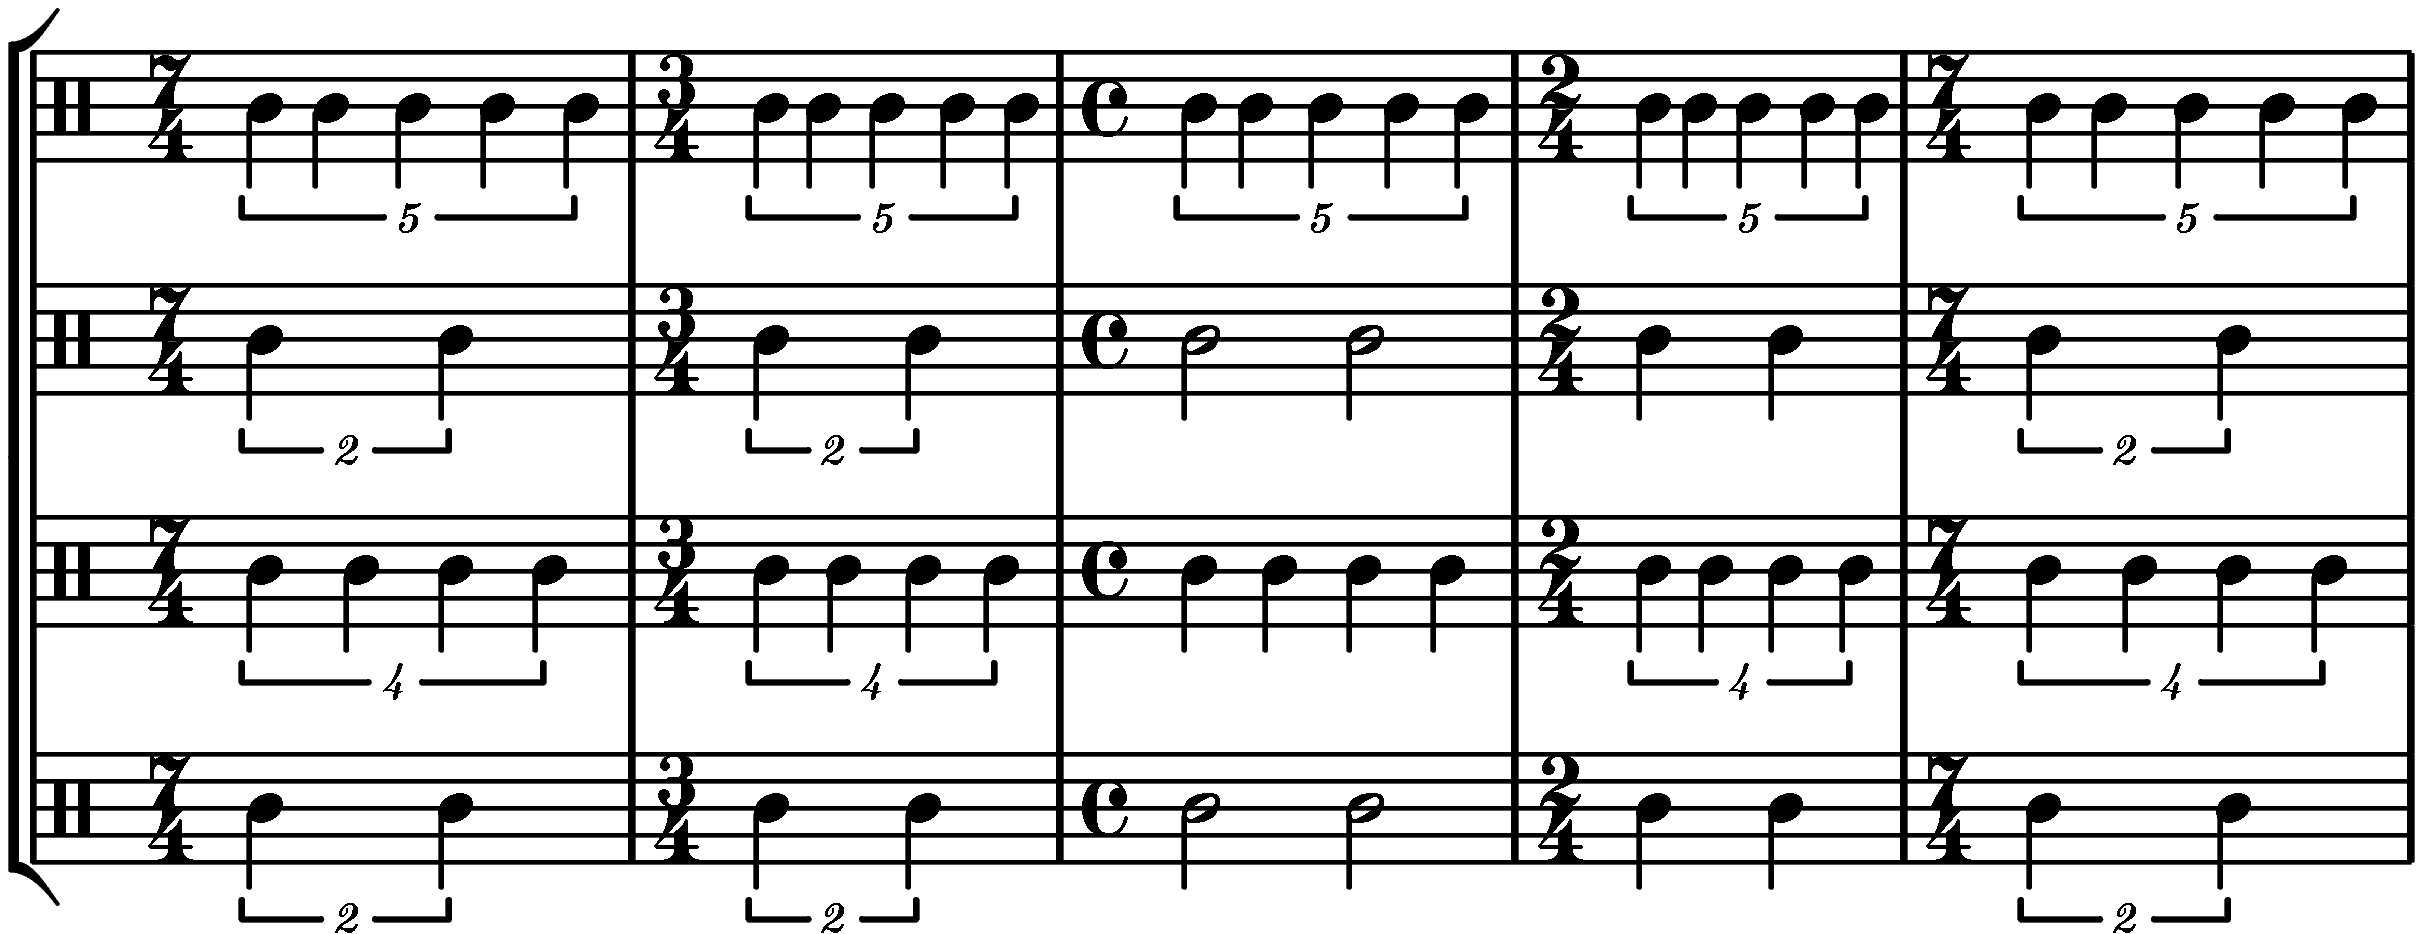
\includegraphics[width=0.75\textwidth]{img/ethsnd/harm}
    \caption[Rhythmic distribution of notes in \emph{etherSound}: Instrument B]{Rhythmic distribution of notes in Instrument B as a
      result of the message ``\emph{Hello, my name is
        Henrik.}''} \label{time2}
  \end{center}
\end{figure}

\subsubsection{Instrument B}
The phrasing of the notes of the second instrument is somewhat more complex than that of Instrument A. This instrument has, at the most,\footnote{As already stated, the maximum number of voices is set based on what the   processing power of the system is.} as many voices as there are words in the message. An example of the rhythmic mapping of notes is shown in Figure \ref{time2}, the origin of which is the message in Table \ref{time}, with the polyphony limited to four voices. For this instrument the number of beats per bar (i.e. per word) is equal to the number of letters per word, including trailing punctuation marks and white space. If there are fewer words than the maximum polyphony, the number of voices is equal to the number of words; the first voice corresponds to the first word, the second voice to the second word and so on. For every bar, each voice has as many potential excitations as there are letters in the corresponding word. After the initial excitation, which will always be played, the likelihood that a given note will be played is related to the life index \emph{and} the global index: if the normalised sum of the local index and the global index is 0.5, half of the excitations will be performed. The amplitude envelope curve for the notes played by this instrument is either of a bell-like character or its inversion, and notes close to the beginning of a bar have a greater likelihood of being emphasised. 

\begin{figure}[!htb]
\begin{center}
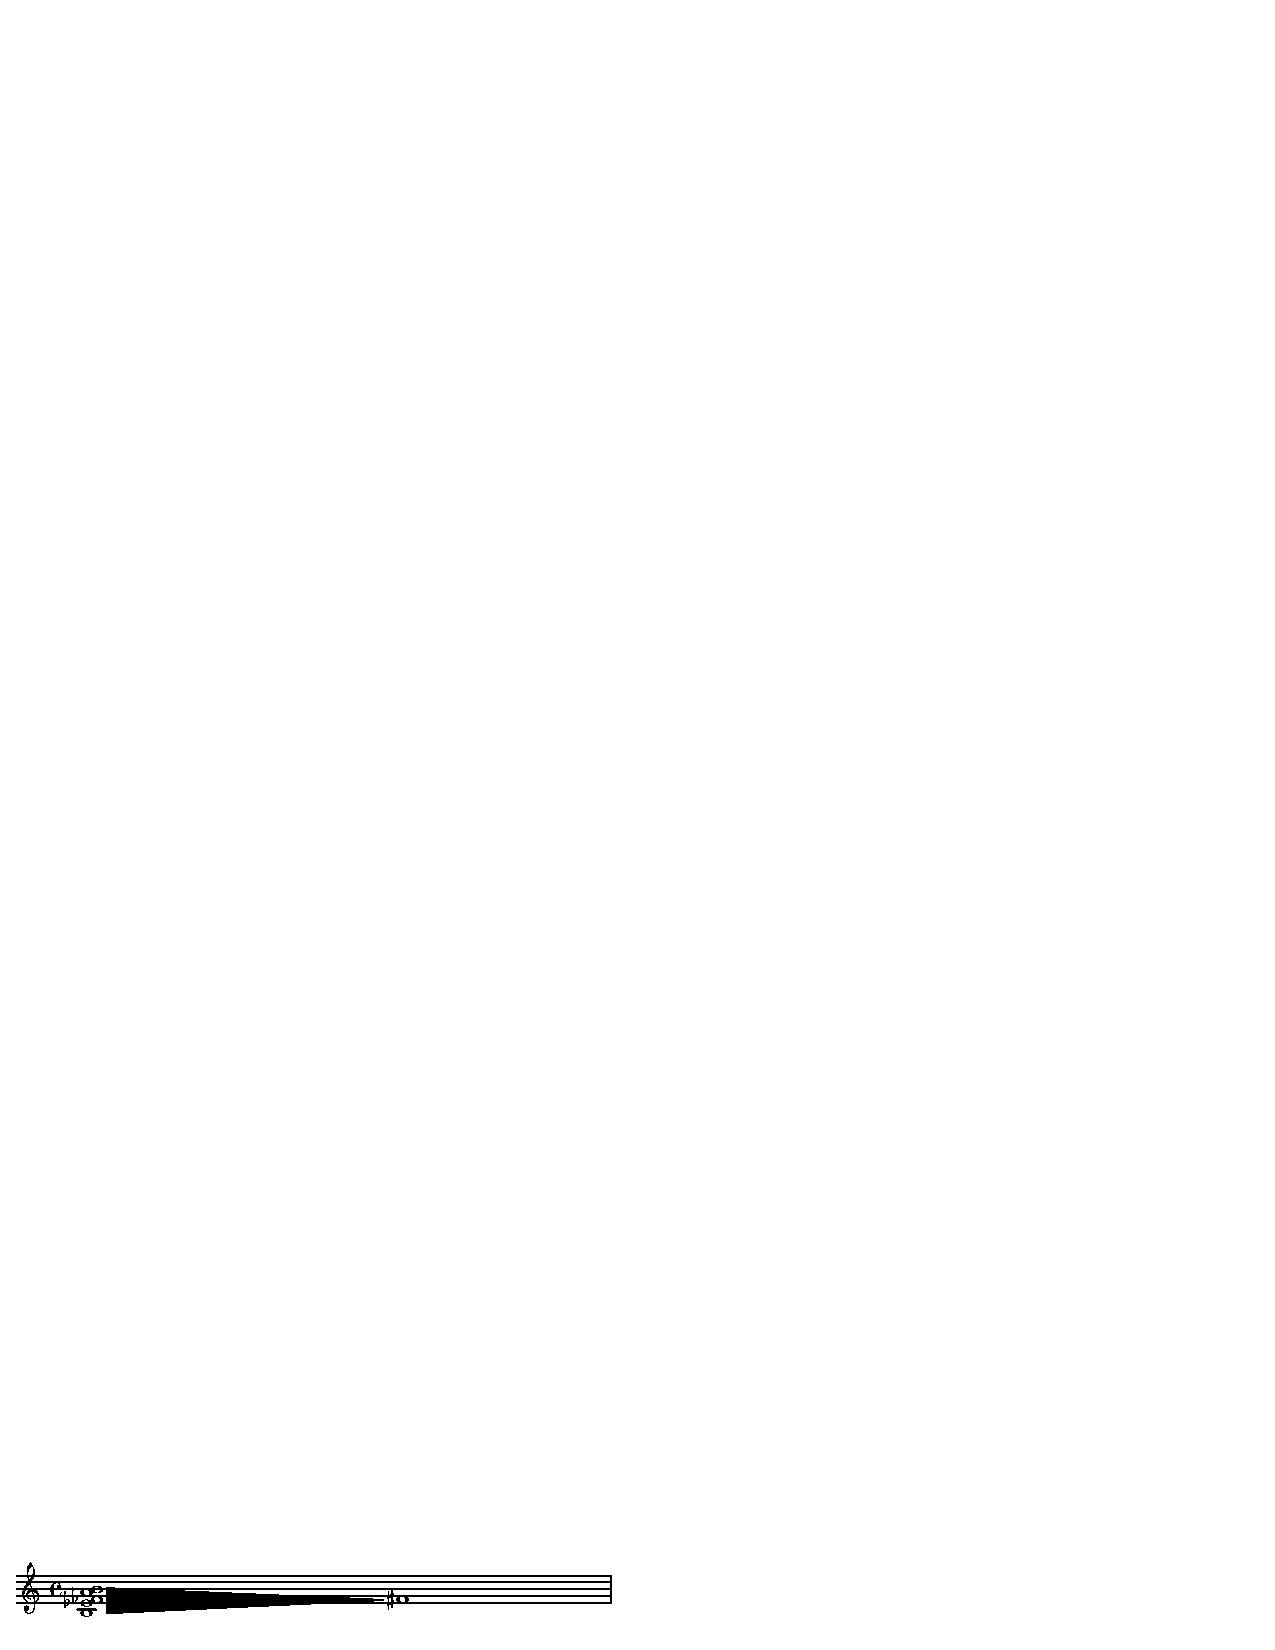
\includegraphics[width=0.75\textwidth]{img/ethsnd/chord}
\caption[Harmony for \emph{etherSound}: Instrument B]{Harmony for Instrument B as a result of the message
  ``\emph{Hello, my name is Henrik.}''.} \label{chord}
\end{center}
\end{figure}

The initial pitches are derived from the occurrence of certain key letters in the originating text.\footnote{For the sake of experiment   and variation, I am changing these 'key notes' for every performance   of \emph{etherSound}.} The first unique occurrence of one of the key letters, searched for from the first letter of the word corresponding to the current voice until the end of the message, becomes the initial pitch for each voice. If none is found, the voice is deleted. The voicing of the initial chord is constructed so that the first voice will be the top note of the chord and consecutive voices will be laid out below this using octave transposition, aiming for the closest possible voicing. 
The exact micro-tonal centre pitch between the highest and lowest note of the initial chord is then calculated (this would be the pitch `D' if the initial chord is a major third up from `C'). After the initial chord has been introduced, all voices begin a virtual glissando toward the centre between the outer limits of the chord, creating micro-tonal variations, ending at a unison.\footnote{The same technique is used in   the composition \emph{Drive} (2003). The score for \emph{Drive}   shows the notation of the instantaneous (approximate) harmony at five consecutive points in time, ending at a B quarter of a tone   sharp.} For each excitation of each voice, the instantaneous value of the corresponding glissando sets the pitch for that excitation. The message from Table \ref{time} would result in the chord shown in Figure \ref{chord}---the initial chord and the glissandi towards the centre pitch---if the max polyphony value is set to five or higher and the `key' characters are mapped by German note names (a to A, b to Bb, c to C, ... ,h to B and s to Eb). 
The timbre of the voices played by this instrument is shaped by the vowels contained in the message and the order in which they appear. For non-real-time processing this is achieved by synthesising the first five formants of the first vowel found in the word corresponding to the current voice and then interpolating between the formant spectrum of the remaining vowels of the message (see Table \ref{vowel}). As this method is very expensive---it requires allocation of five times as many voices---a cheaper alternative was used in the first real time versions of \emph{etherSound}. By modulating the formant centre frequency of one single FOF voice using frequency modulation with the carrier and index signal frequencies derived from the vowel interpolation described above, the effect of moulding the spectrum in a way related to the content of the message is retained. In the latest version the two methods are combined in order to achieve a greater sonic variation---all five formants are synthesised for every note and the formant centre frequencies of some of the notes are also modulated. 
\subsection{Sound event generation and synthesis---conclusion} The two instruments offer different interpretations of the message played back in parallel. As Instrument A performs a linear displacement within the message, Instrument B gives a snapshot image of the entire text at once, an image which gradually dissolves over time. Metaphorically speaking, one instrument is modelling the discrete words and characters as they appear in time, the objective flow of the components of the message, and the other deals with the continuous meaning, or subjective understanding, of the message as it is interpreted in its entirety. Although the result can be rather complex and abstract it is my intention that certain conceptual elements of the input should be retained in the output. In the following section I will reflect on the issue of interaction within the context of \emph{etherSound} and to what extent my intentions of input-output correlation can be said to have been fulfilled. 

%\newpage
\begin{landscape}
\centering
\begin{table}[!pt]
\begin{tabularx}{\linewidth}{|p{.8in}|X|X|X|X|X|X|X|X|X|X|X|X|X|X|X|X|X|X|X|X|X|X|X|X|X|}
\hline
&H & E & L & L & O &,& &M&Y& &N&A&M&E& &I&S& &H&E&N&R&I&K&.\\
\hline
\textit{bar}&\multicolumn{7}{|l|}{1} & \multicolumn{3}{|l|}{2} & \multicolumn{5}{|l|}{3} & \multicolumn{3}{|l|}{4} & \multicolumn{7}{|l|}{5}\\
\hline
\textit{beats per bar}&\multicolumn{7}{|c|}{3} & \multicolumn{3}{|c|}{1} & \multicolumn{5}{|c|}{2} & \multicolumn{3}{|c|}{1} & \multicolumn{7}{|c|}{3}\\
\hline
\textit{subdivision}&\multicolumn{2}{|c|}{2} & \multicolumn{3}{|c|}{3} & \multicolumn{2}{|c|}{2} & \multicolumn{3}{|c|}{3} & \multicolumn{2}{|c|}{2} & \multicolumn{3}{|c|}{3} & \multicolumn{3}{|c|}{3} & \multicolumn{2}{|c|}{2} & \multicolumn{3}{|c|}{3} & \multicolumn{2}{|c|}{2}\\
\hline
\textit{accents}& & \textgreater & & &\textgreater & & & & \textgreater& & & \textgreater& &\textgreater & &\textgreater& & & & \textgreater& & &\textgreater&\textgreater& \\
\hline
\end{tabularx}
\caption[Rhythmic distribution of notes in Instrument A.]{Rhythmic distribution of notes in Instrument A. Influence of vowels on four consecutive voices of Instrument B.} \label{time}
\end{table}

\centering
\begin{table}[!pt]
\begin{tabularx}{\linewidth}{|p{.8in}|X|X|X|X|X|X|X|X|X|X|X|X|X|X|X|X|X|X|X|X|X|X|X|X|X|}
\hline
&H & E & L & L & O &,& &M&Y& &N&A&M&E& &I&S& &H&E&N&R&I&K&.\\
\hline
\textit{voice 1}&\multicolumn{3}{|c|}{E} & \multicolumn{3}{|c|}{O} & \multicolumn{3}{|c|}{Y} & \multicolumn{3}{|c|}{A} & \multicolumn{3}{|c|}{E} & \multicolumn{3}{|c|}{I} & \multicolumn{3}{|c|}{E} & \multicolumn{4}{|c|}{I}\\
\hline
\textit{voice 2}& \multicolumn{4}{|c|}{Y} & \multicolumn{4}{|c|}{A} & \multicolumn{4}{|c|}{E} & \multicolumn{4}{|c|}{I} & \multicolumn{4}{|c|}{E} & \multicolumn{5}{|c|}{I}\\
\hline
\textit{voice 3}& \multicolumn{5}{|c|}{A} & \multicolumn{5}{|c|}{E} & \multicolumn{5}{|c|}{I} & \multicolumn{5}{|c|}{E} & \multicolumn{5}{|c|}{I}\\
\hline
\textit{voice 4}& \multicolumn{8}{|c|}{I} & \multicolumn{8}{|c|}{E} & \multicolumn{9}{|c|}{I}\\
\hline
\end{tabularx}
\caption{Influence of vowels on four consecutive voices of Instrument B.} \label{vowel}
\end{table}

\end{landscape}

%%% Local Variables: 
%%% mode: latex
%%% TeX-master: "../ImprovisationComputersInteraction"
%%% End: 
